\intro
В настоящее время существует множество задач, требующих бесконтактного метода измерений: ориентирование в пространстве, измерение объектов, реконструкция объектов, сбор биометрических данных, реверс-инжиниринг, а также дизайн и творчество. Подобных задач с каждым годом становится всё больше, и таким образом растёт важность 3D-сканирования и следовательно необходимость эффективных алгоритмов, решающих конкретную задачу. Кроме того, некоторые задачи требуют уникальных встроенных решений, что представляет собой как правило ещё и конструкторскую задачу.

Одним из конкретных применений такой технологии является фигурное нанесение глазури на различные кондитерские изделия. На данный момент такая операция как правило выполняется вручную, что означает высокую стоимость, длительное производство и низкую повторяемость. Автоматизация этого процесса происходит обычно на крупных предприятиях, где производят большие партии однотипных кондитерских изделий.

Относительно недавно стали появляться автоматизированные комплексы для нанесения рисунков на различные кондитерские изделия, однако они всё равно ограничены конкретными видами изделий (например, плоские крекеры). Такие комплексы работают по принципу 3D-принтера или ЧПУ-станка. Они печатают в одной плоскости, не имея возможности наносить материал с учётом отклонений формы, не говоря уже об изделиях сложной формы, таких как овсяное печенье, кексы, торты и т.д., у которых форма в общем случае не только не плоская, но и обладает множеством искривлений, выпуклостей и впадин. Данное обстоятельство мешает автоматизации нанесения произвольных рисунков на произвольные изделия.

Данная работа посвящена разработке модуля 3D-сканирования для кондитерского принтера, что позволит наносить рисунки на произвольные изделия. Разработка основывается на базе прототипа системы автоматического фигурного нанесения пищевой пасты в который модуль необходимо встроить. Прототип представляет из себя принтер закрытого типа с подвижным печатающим узлом и статичным столом, на котором располагаются кондитерские изделия.

\begin{figure}[!ht]\label{pic:printer_start}
    \centering
    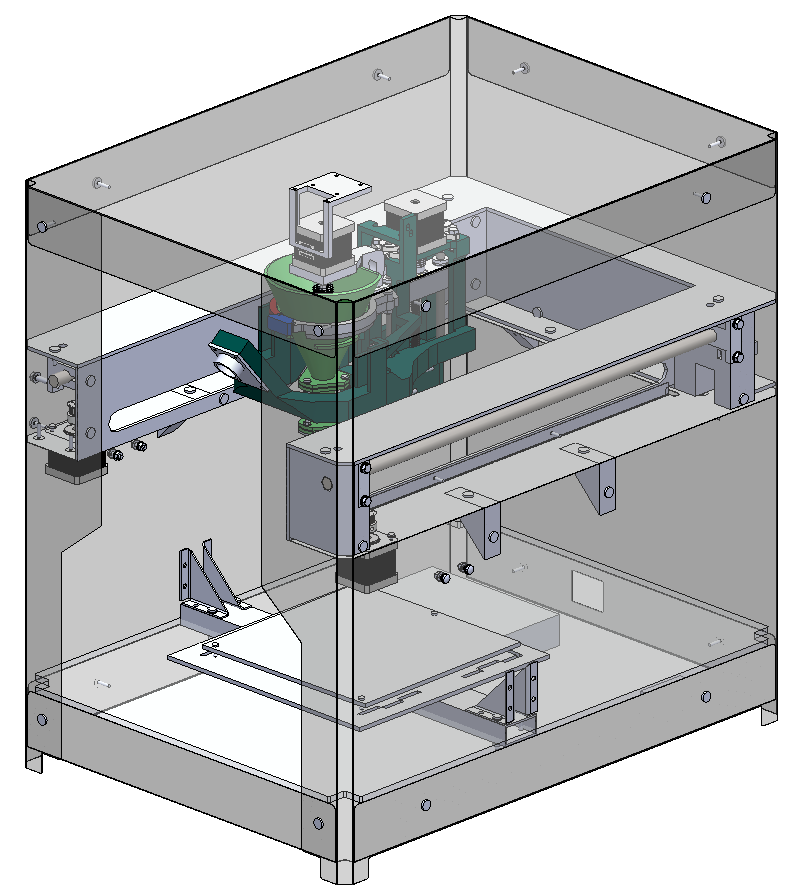
\includegraphics[width=0.5\linewidth]{printer_start}
    \caption{Прототип системы автоматического фигурного нанесения пищевой пасты}
\end{figure}

В направлении технического зрения для прототипа уже была проделана некоторая работа, однако, как показала практика, этого было недостаточно в виду чего потребовалась разработка нового модуля и соответствующего алгоритма для его работы.

Алгоритм должен решать следующие задачи:
\begin{itemize}
    \item получение облака точек рабочей зоны
    \item обнаружение объектов и их положений в облаке точек
    \item генерация gcode произвольного рисунка с учётом облака точек
\end{itemize}

Новый модуль должен удовлетворять следующим требованиям:
\begin{itemize}
    \item рабочая зона $ 200 \times 200 \text{ мм}$
    \item точность $ \pm 0.5 \text{ мм} $
    \item время обработки данных не более 30 секунд
    \item минимальная стоимость
\end{itemize}
